% PRISM / CAPOPM paper skeleton (Stage J)
\documentclass[11pt]{article}
\usepackage[margin=1in]{geometry}
\usepackage{amsmath, amssymb}
\usepackage{graphicx}
\usepackage{hyperref}
\usepackage{booktabs}

\title{PRISM: A Reproducible Pipeline for Proxy-Evidence Bayesian Inference in Market Microstructure}
\author{PRISM Research Team}
\date{\today}

\begin{document}
\maketitle

\begin{abstract}
We present PRISM, a reproducible research pipeline for evaluating CAPOPM-style Bayesian parimutuel inference under synthetic data generating processes and real-market \emph{proxy evidence} derived from market microstructure. The package emphasizes auditability, explicit guardrails against overclaiming, and artifact-based reproducibility. Real-data results in this repository are illustrative demonstrations and do not constitute theorem validation.
\end{abstract}

\section{Introduction}
% Motivation and framing.

\section{Related Work}
% Bayesian market inference, calibration, microstructure evidence.

\section{Theoretical Framework}
This manuscript is aligned to \texttt{THEORY\_APPENDIX.MD}. We use Beta--Binomial conjugacy and associated posterior predictive quantities.

\section{Model Definition}
Define the latent probability $p \in (0,1)$, prior $p \sim \mathrm{Beta}(\alpha_0,\beta_0)$, and evidence counts $(y,n)$.

\section{Evidence Aggregation}
Evidence is aggregated from a canonical evidence tape with entries (side, size, timestamp). Counts are:
\begin{align}
 y &= \sum_{i: \text{YES}} w_i,\\
 n &= \sum_i w_i.
\end{align}

\section{Posterior Inference}
Posterior update:
\begin{align}
 \alpha_{post} &= \alpha_0 + y,\\
 \beta_{post} &= \beta_0 + (n-y).
\end{align}
Posterior mean and variance (Proposition 5):
\begin{align}
 \mathbb{E}[p\mid \cdot] &= \frac{\alpha_{post}}{\alpha_{post}+\beta_{post}},\\
 \mathrm{Var}(p\mid \cdot) &= \frac{\alpha_{post}\beta_{post}}{ (\alpha_{post}+\beta_{post})^2(\alpha_{post}+\beta_{post}+1)}.
\end{align}

\section{Experimental Setup}
Summarize synthetic tiers and real-data artifact campaigns.

\section{Real-Data Validation (Proxy Evidence)}
Describe Databento schema (trades) and experiment grids (short-horizon grid + expanded validation across slices/windows).

\section{Predictive Evaluation}
Describe proxy outcome: future trade-price direction at horizons 1/5/15 minutes. Scoring uses Brier and predictive log loss.

\section{Baseline Comparisons}
Compare PRISM posterior mean to imbalance estimator (expected equivalence in this configuration), plus naive Beta baseline and a descriptive logistic smoother.

\section{Limitations}
Proxy evidence disclaimer; dependence and effective sample size; latent regime unobservability; no dominance claims.

\section{Conclusion}

\clearpage
\section*{Figures}
\begin{figure}[h]
\centering
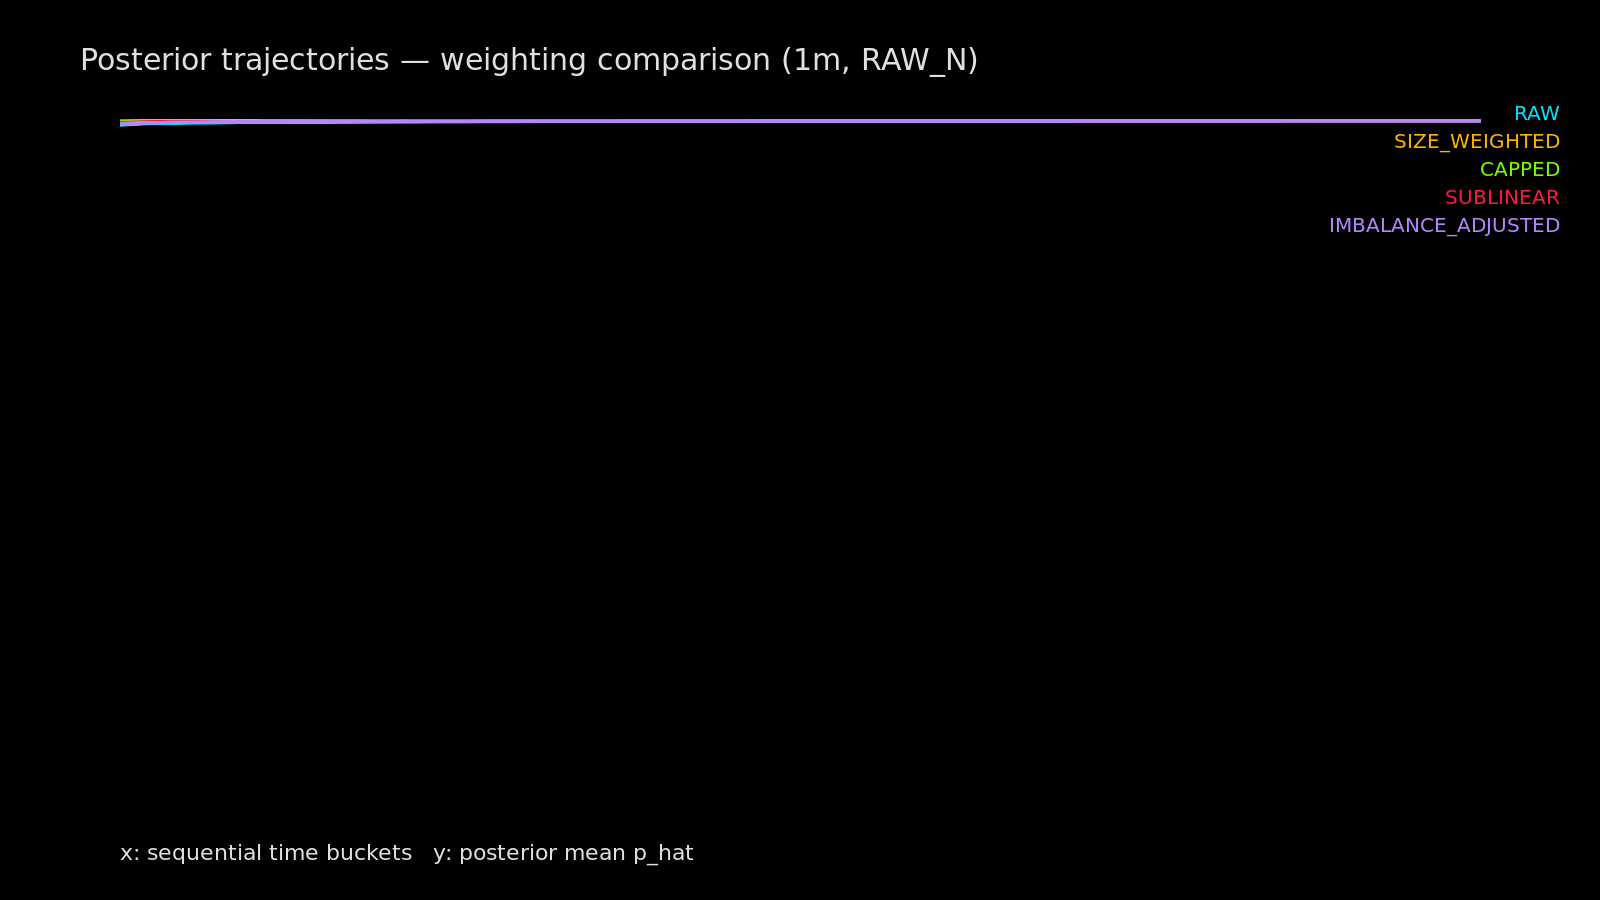
\includegraphics[width=0.95\linewidth]{../figures/fig2_posterior_evolution.png}
\caption{Posterior trajectory comparison (illustrative).}
\end{figure}

\begin{figure}[h]
\centering
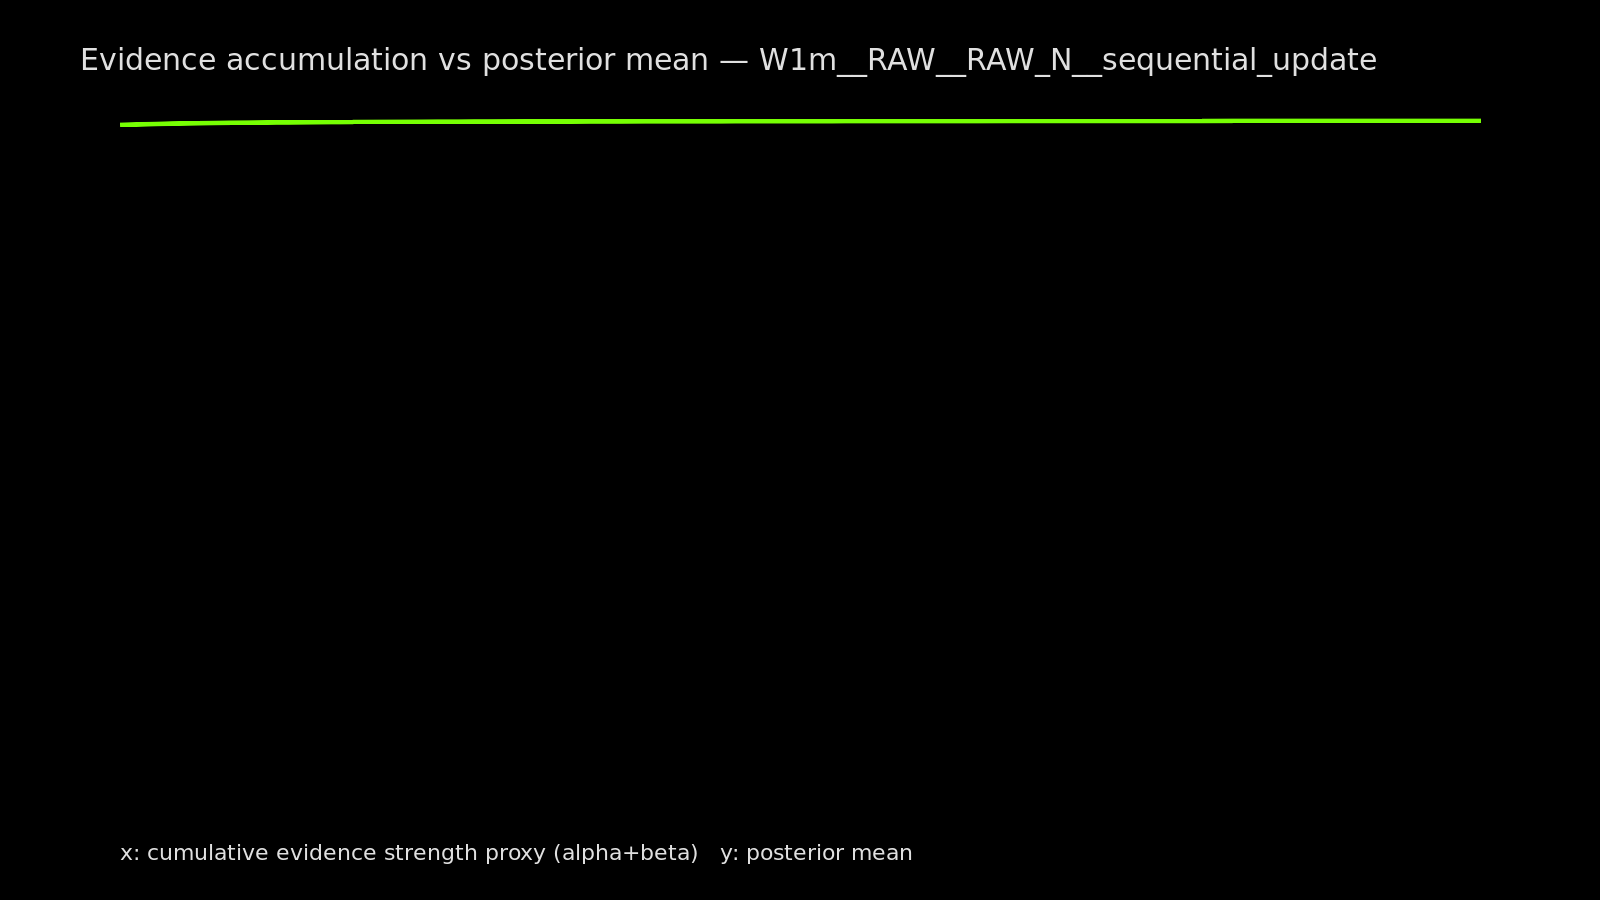
\includegraphics[width=0.95\linewidth]{../figures/fig3_evidence_accumulation.png}
\caption{Evidence accumulation vs posterior mean (illustrative).}
\end{figure}

\begin{figure}[h]
\centering
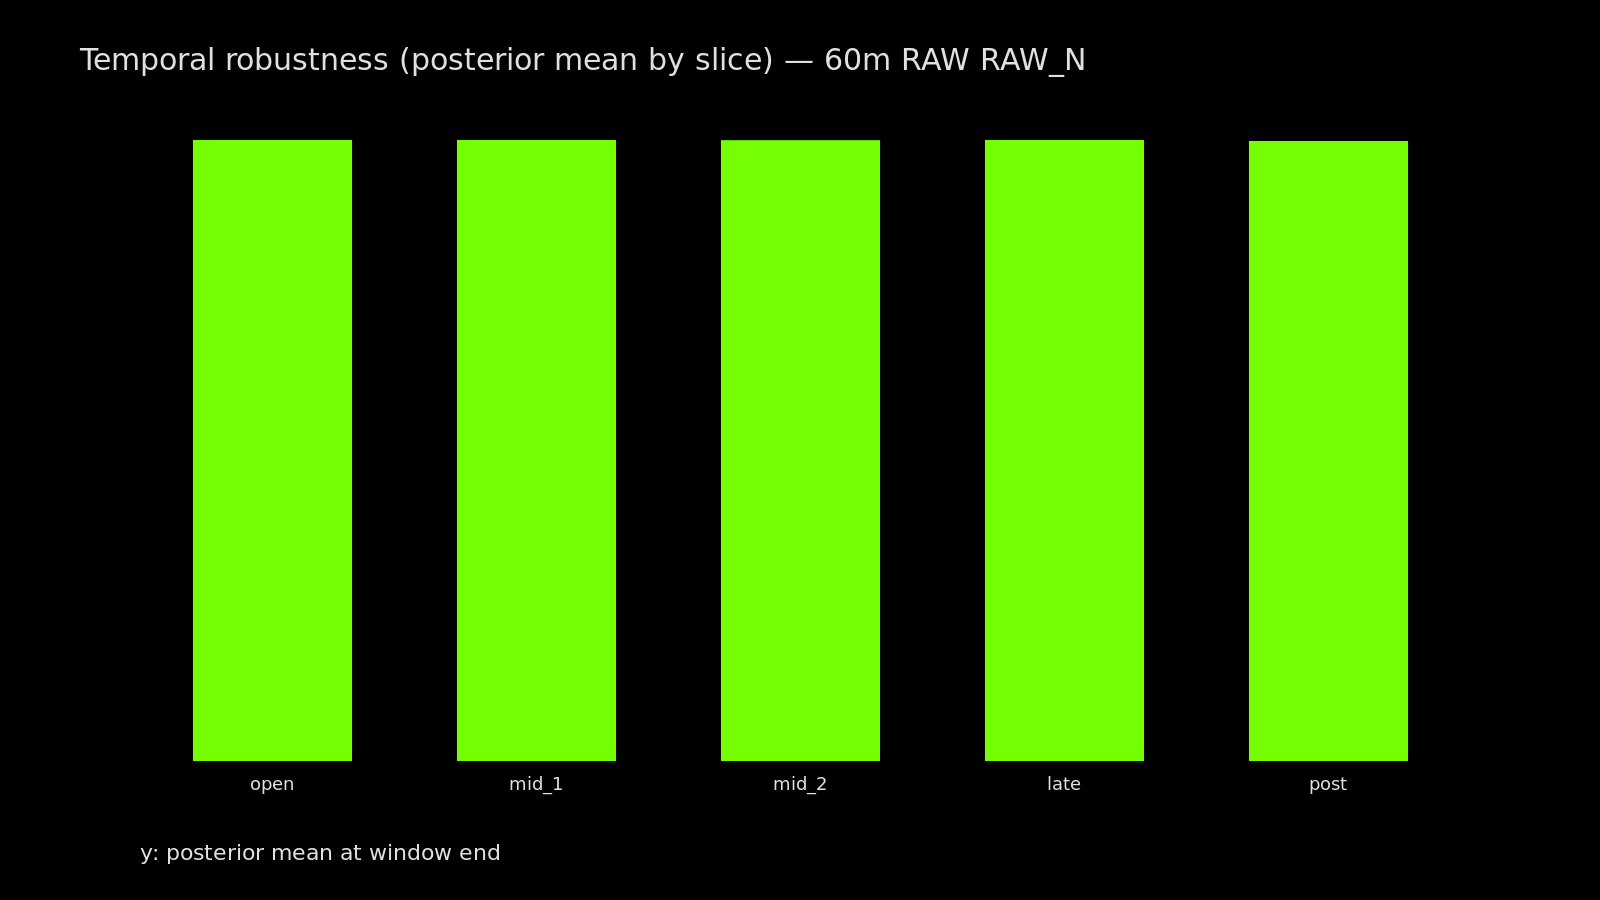
\includegraphics[width=0.95\linewidth]{../figures/fig4_temporal_robustness.png}
\caption{Temporal robustness across slices (illustrative).}
\end{figure}

\begin{figure}[h]
\centering
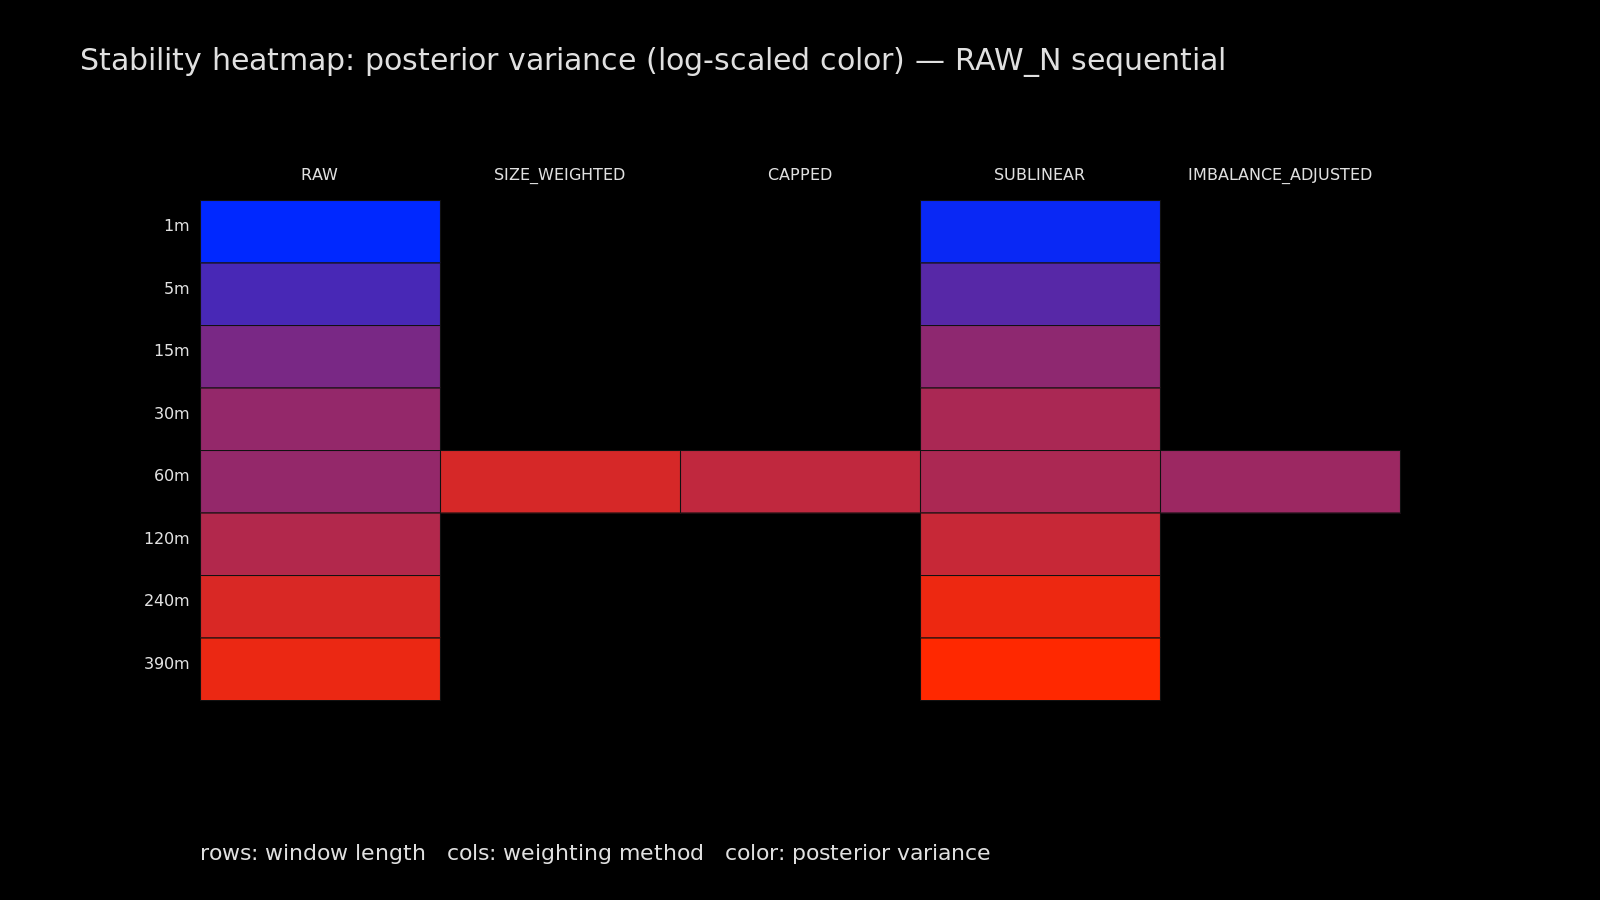
\includegraphics[width=0.95\linewidth]{../figures/fig5_weighting_variance_heatmap.png}
\caption{Variance heatmap across windows and weighting (illustrative).}
\end{figure}

\begin{figure}[h]
\centering
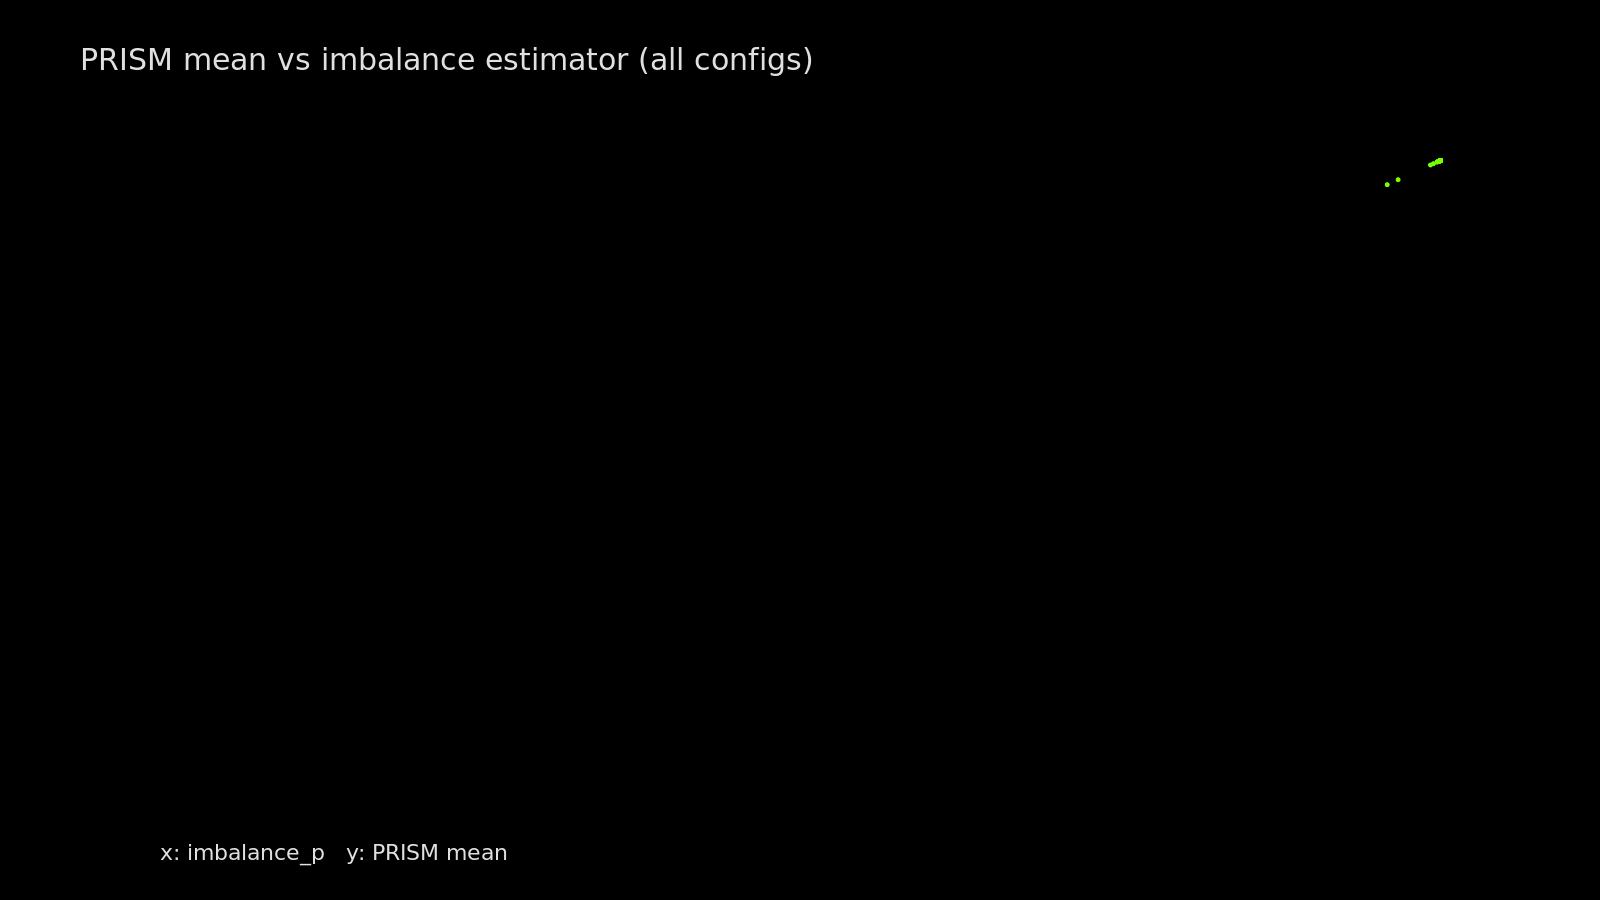
\includegraphics[width=0.95\linewidth]{../figures/fig6_baseline_comparison.png}
\caption{PRISM vs imbalance baseline (descriptive).}
\end{figure}

\begin{figure}[h]
\centering
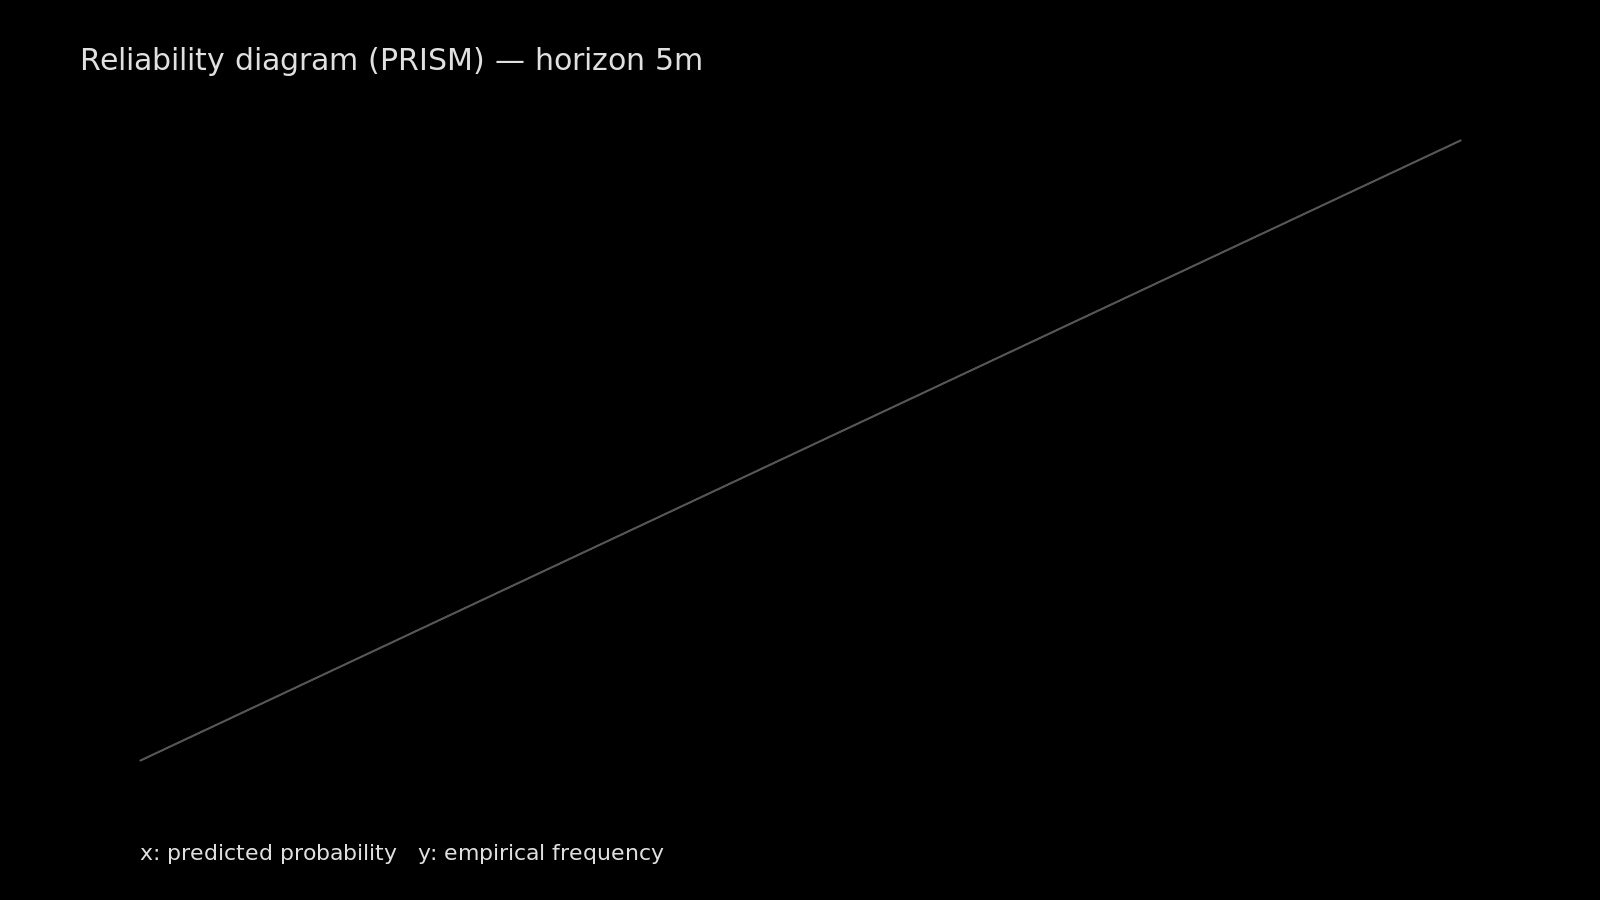
\includegraphics[width=0.95\linewidth]{../figures/fig7_predictive_reliability.png}
\caption{Predictive reliability diagram for proxy outcome (illustrative).}
\end{figure}

\begin{figure}[h]
\centering
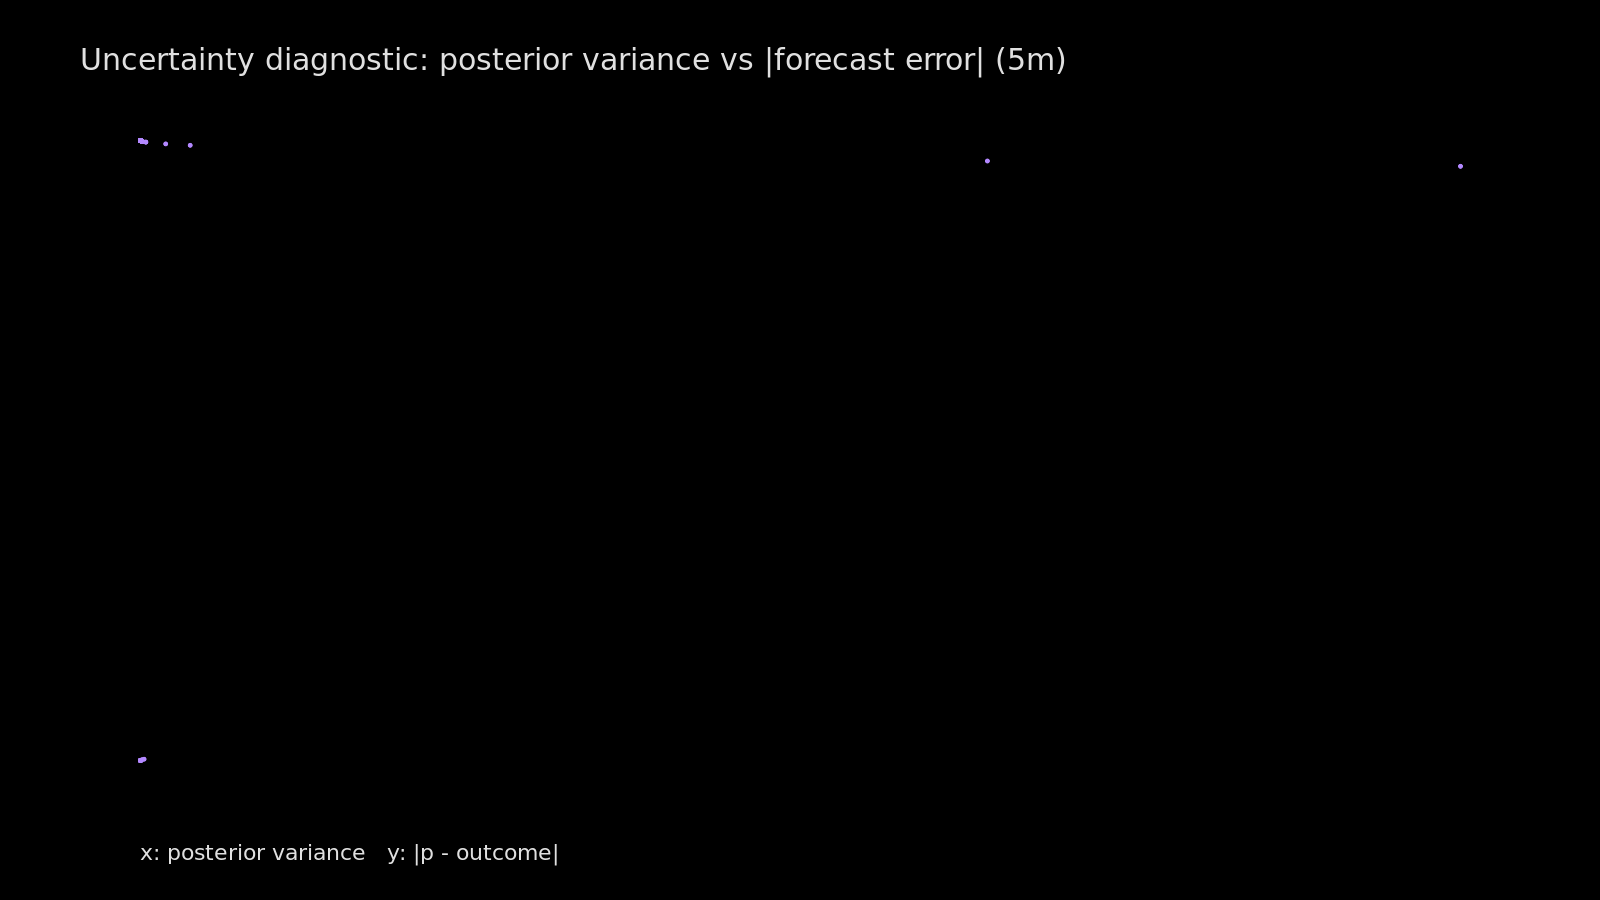
\includegraphics[width=0.95\linewidth]{../figures/fig8_uncertainty_vs_error.png}
\caption{Posterior variance vs forecast error (proxy; descriptive).}
\end{figure}

\end{document}
